\chapter{Der Photoeffekt}
%Some parts will be used later

%Die Grundlagen werden später gelöscht und der Inhalt in die Durchführung/Auswertung eingebaut
%\section{Grundlagen}
%\subsection{Photoeffekt}
%Der Photoeffekt tritt bei Ionisierung von Atomen durch Lichteinstrahlung, wobei die Energie der Valenzelektronen so weit ansteigt, dass sie das Potential des Atoms verlassen können. Dies geschieht nur, wenn das Licht eine Mindestenergie erreicht, die der Tiefe des Elektronenpotentials entspricht. Die Energie des Lichts \(E\) hängt mit ihrer Frequenz \(\nu\) durch die Beziehung \(E = \nu h\) zusammen, wobei \(h\) das Plancksche Wirkungsquantum darstellt. 
%\subsection{Funktionsweise einer Photozelle}

%\paragraph{Aufbau}
%Eine Photozelle besteht aus einer Ringanode und einer Kathode, welche mit Licht beleuchtet
%wird. Die Anode und die Kathode bestehen aus unterschiedlichen Materialien.


%\begin{figure}[htbp]
%    \centering
%    \includegraphics[width=0.75\textwidth]{figs/anlegen_aeuß_potential.png}
%    \caption{ Kontaktpotential $-eU_{KA}$ \cite{praktikum}}
%    \label{fig:potential ext}
%\end{figure}
%\FloatBarrier

%\begin{figure}[htbp]
%    \centering
%    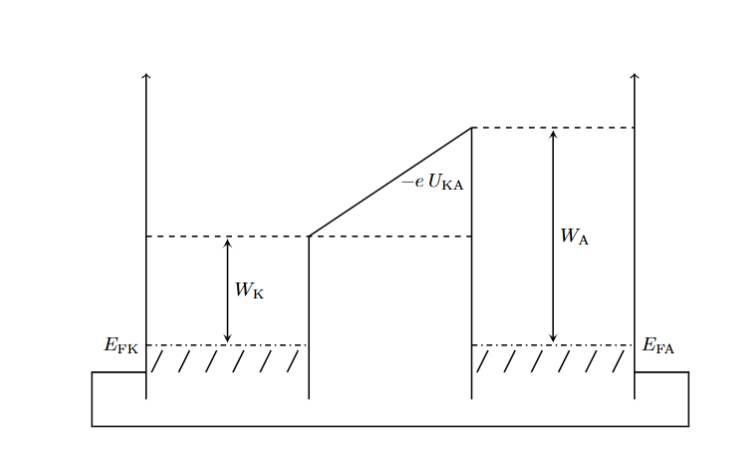
\includegraphics[width=0.75\textwidth]{figs/kontaktpotential_kurzgeschl_elektroden.png}
%    \caption{  Potential dass von der Gegenspannung
%$-eU_G$ induziert wird\cite{praktikum}}
%    \label{fig:potential kurzg.}
%\end{figure}
%\FloatBarrier

%\paragraph{Wirkung}
%\begin{figure}[htbp]
%    \centering
%    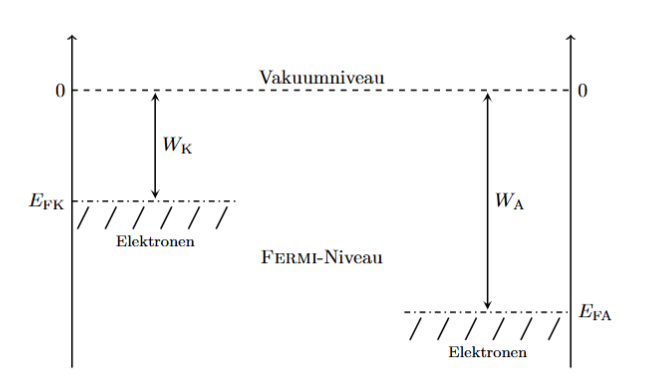
\includegraphics[width=0.75\textwidth]{figs/baenderschema_kathode_anode.png}
%    \caption{ Ferminiveaus von Kathode und Anode mit Austrittsarbeit $W_A$ \cite{praktikum}}
%    \label{fig:kathode-anode}
%\end{figure}
%\FloatBarrier
%Das Anodenmaterial weist eine höhere Austrittsarbeit auf als das Kathodenmaterial, wodurch beim Kontakt eine Potentialdifferenz zwischen ihren Ferminiveaus entsteht. Diese Differenz verstärkt sich, wenn eine zusätzliche Gegenspannung zwischen Anode und Kathode angelegt wird.\\
%Die durch das Licht herausgelösten Elektronen gewinnen entsprechend seiner Energie kinetische Energie und bewegen sich zur Anode, wodurch ein messbarer Strom entsteht. Die angelegte Gegenspannung verlangsamt die Elektronen und wird schrittweise erhöht, bis kein Photostrom mehr nachweisbar ist – also die Elektronen aus dem Anodenmaterial nicht mehr die Anode erreichen.
%\paragraph{Photostromverlauf}
%\paragraph{Austrittsarbeit}
%\paragraph{Kontaktpotential}




%bleibt da, den Aufbau erläutern
\section{Aufbau}
\begin{figure}[htbp]
    \centering
    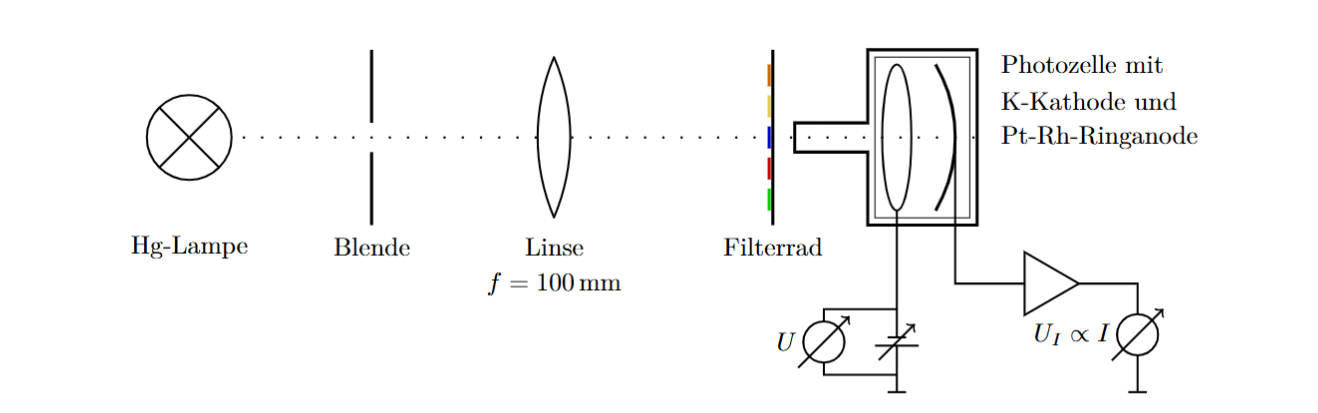
\includegraphics[width=0.75\textwidth]{figs/Aufbau_plank_wirkungsquantum.png}
    \caption{Aufbau für die Messung des Photoeffektes  \cite{praktikum}}
    \label{fig:aufbau teil 1}
\end{figure}
\FloatBarrier
Links ist die Hg-Lampe zu sehen, in der
Mitte Optik-Elemente zum Fokussieren und Filtern des Lichtes und rechts ist die Photozelle
mit Gegenspannung und Strommessung.\\
Die Quecksilber-Spektrallampe und die Photozelle 
werden gemäß Abbildung \ref{fig:aufbau teil 1} 
gegenüberliegend auf dem Reiter angeordnet. 
Eine Irisblende vor der Lampe ermöglicht die 
Regulierung der Lichtintensität. Eine Linse 
mit einer Brennweite von f=100 mm wird in 
diesem Abstand vor die Blende positioniert,
 sodass sie das Licht parallel auf den 
 nachfolgenden Interferenzfilter mit fünf 
 Filtern sowie eine zusätzliche Blende lenkt.

%---------------------------------------------------------------
\section{Durchführung}

Eine Abschirmvorrichtung mit einem 
röhrenförmigen Element verhindert Streulicht. 
Ein Lichtfleck wird gezielt auf die Kathode 
projiziert, ohne ,dass die Anode beleuchtet wird.

Wenn Photonen aus der Hg-Lampe auf die Photokathode treffen, interagieren sie mit den Elektronen in dieser und überträgt dabei seine gesamte Energie $E = h\nu$
auf eines der Elektronen. Falls die übertragene Energie größer als die Austrittsarbeit $W_A$ ist,dann kann sich das Elektron aus der Kathode lösen und zur Ringanode gelangen. Dadurch ensteht ein Stromfluss:der Photostrom $I_{ph}$.
Durch den Einsatz der Gegenfeldmethode wird die maximale kinetische Energie, die die Elektronen beim verlassen der Kathode besitzen, bestimmt.

Bei dieser Methode wird eine Gegenspannung $U_G$ zwischen Kathode und Anode angelegt, wodurch die Kathode im Vergleich zur Anode ein positives Potential erhält.
Das dadurch erzeugte elektrische Feld verlangsamt die emittierten Elektronen auf ihrem Weg zur Anode, wodurch der Photostrom reduziert wird. Sobald die Grenzspannung $U_0$ erreicht ist, kommt der Photostrom vollständig zum Erliegen. 
Dies bedeutet, dass selbst die energiereichsten Elektronen die Anode nicht mehr erreichen können. In diesem Fall gilt die Beziehung: 
$E_{kin,max} = eU_0$.

Man lässt das Gegenfeld mit Hilfe einer variablen Spannungsquelle, welche sich zwischen der Kathode und der Anode befindet, ansteigen.
Man erweitert die Schaltung mit Hilfe eines Spannungsteilers (Abbildung \ref{fig:spannungsteiler}) aus einem $330\Omega$ und $100\Omega$ Widerstandes um den Messbereich zu skalieren und genauere Messungen durchzuführen.
\begin{figure}[htbp]
    \centering
    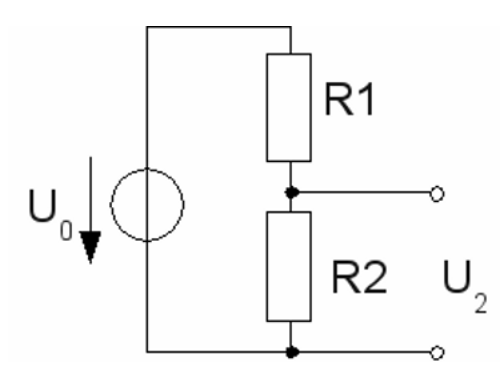
\includegraphics[width=0.3\textwidth]{figs/Spannungsteiler.png}
    \caption{ Spannungsteiler \cite{Spannungsteiler}}
    \label{fig:spannungsteiler}
\end{figure}
\FloatBarrier
Die verwendete Spannungsquelle kann Spannungen von 0\,V bis 12\,V bereitstellen. 
Der Photostrom erreicht jedoch bereits bei deutlich geringeren Gegenspannungen seinen Nullpunkt, typischerweise im Bereich von wenigen Volt. 
Für die Messung der Grenzspannung $U_0$ genügt daher ein kleiner Teil des gesamten Spannungsbereichs. 
Die feine Justierung der Gegenspannung ist entscheidend, um den Punkt zu bestimmen, an dem der Photostrom gerade verschwindet.\\
Es gilt folgender Zusammenhang zwischen der abgefangenen Spannung $U_2$, den Widerständen $R_1 = 330 \Omega, R_2 = 100 \Omega$ und $U_0$:
\begin{equation}
  U_2 = \frac{R_2}{R_1 + R_2}\,U_0
\end{equation}\\
Sommit wird der Spannungsbereich auf [0, 2{,}8]\,V skaliert.\\

Der Anodenstrom wird über einen Messverstärker erfasst, 
wobei eine zum Strom proportionale Spannung mit einem 
Digitalmultimeter (DMM) gemessen wird. Die Gegenspannung 
stammt aus einem 12V-Gleichspannungsnetzteil, 
wobei der negative Pol mit der Anode verbunden ist, 
um die Elektronen abzubremsen. Diese Spannung wird 
mit einem weiteren DMM gemessen.\\
Dieser Vorgang wird für je eine unterschiedliche Wellenlänge
$\lambda$ des Lichtes zwei mal wiederholt (zum Ausgleich der Schwankungen), wobei die
Wellenlängen mit Hilfe von Interferenzfiltern
einstellbar sind.

%--------------------------------------------------------------

\subsection{Energiebilanz der Photoelektronen}
Ein Elektron, dass sich in der Kathode befindet, absorbiert ein Photon mit der Energie $E = h\nu$ und verlässt die Kathode, wenn die Energie des Photons größer ist als eine bestimmte Potentialdifferenz sein: die Austrittsarbeit $W_K$.
In Abbildung \ref{fig:kathode-anode}, \ref{fig:potential ext} und \ref{fig:potential kurzg.} sind die Austrittsarbeit $W_K$ der Kathode und die Austrittsarbeit $W_A$ der Anode für unterschiedliche elektrische Anordnungen dargestellt.\\ %nachprüfen ob Referenzen gut gesetzt sind


\begin{figure}[htbp]
    \centering
    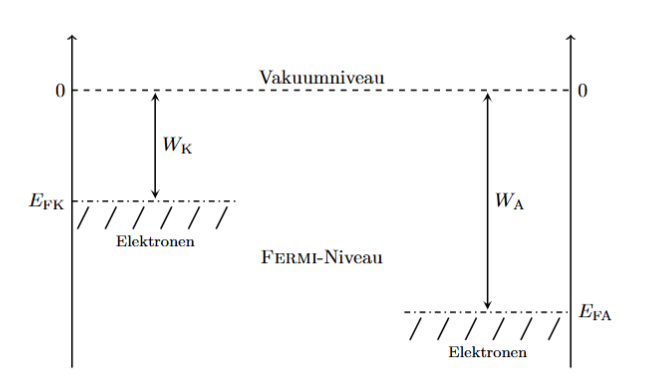
\includegraphics[width=0.75\textwidth]{figs/baenderschema_kathode_anode.png}
    \caption{ Ferminiveaus von Kathode und Anode mit Austrittsarbeit $W_A$ \cite{praktikum}}
    \label{fig:kathode-anode}
\end{figure}
\FloatBarrier

\begin{figure}[htbp]
    \centering
    \includegraphics[width=0.75\textwidth]{figs/anlegen_aeuß_potential.png}
    \caption{ Kontaktpotential $-eU_{KA}$ \cite{praktikum}}
    \label{fig:potential ext}
\end{figure}
\FloatBarrier

\begin{figure}[htbp]
    \centering
    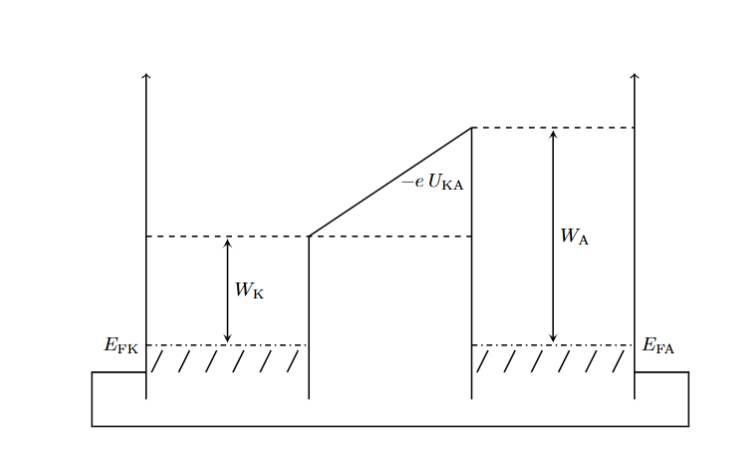
\includegraphics[width=0.75\textwidth]{figs/kontaktpotential_kurzgeschl_elektroden.png}
    \caption{  Potential dass von der Gegenspannung
$-eU_G$ induziert wird\cite{praktikum}}
    \label{fig:potential kurzg.}
\end{figure}
\FloatBarrier


Laut der Abbildung der Ferminiveaus \ref{fig:kathode-anode} 
gilt für die Energiebilanz:
\begin{equation}
    E = h\nu = W_K + eU_{KA} + eU_{G,0} 
    = W_K + W_A - W_K + eU_{G,0} 
    = W_A + eU_{G,0}
\end{equation}\\
Aus der Frequenz des Lichtes können 
schließlich
die Austrittsarbeit der Anode $W_A$ und 
das Planck’sche Wirkungsquantum h bestimmt 
werden:
\begin{equation}
    eU_{G,0} = h\nu - W_A
\end{equation}
\section{Abschätzung des Plankschen Wirkungsquantums und der Austrittsarbeit}
\subsection[Bestimmung der Grenzspannung U0]{Bestimmung der Grenzspannung U\textsubscript{0}}
\subsection[Bestimmung des Plankschen Wirkungsquantums h]{Bestimmung des Plankschen Wirkungsquantums h}
\begin{table}[H]
\centering
\resizebox{0.75\columnwidth}{!}{%
\begin{tabular}{|c|c|c|c|}
\hline
$\lambda$ [\si{\nano\metre}] & $\nu$ [\si{\hertz}] & $\overline{U_0}$ [\si{\milli\volt}] & $\Delta \overline{U_0}$ [\si{\milli\volt}] \\ \hline
\SI{365.00}{\nano\metre} & \num{8.21e14} & \num{2124.19} & \num{45.39} \\ \hline
\SI{405.00}{\nano\metre} & \num{7.40e14} & \num{1605.23} & \num{47.04} \\ \hline
\SI{463.00}{\nano\metre} & \num{6.47e14} & \num{1341.51} & \num{57.42} \\ \hline
\SI{546.00}{\nano\metre} & \num{5.49e14} & \num{638.22}  & \num{59.13} \\ \hline
\SI{578.00}{\nano\metre} & \num{5.19e14} & \num{458.70}  & \num{24.80} \\ \hline
\end{tabular}%
}
\caption{Gemittelte Abbrems­spannungen $\overline{U_0}$ und deren Unsicherheiten gegen die jeweiligen Frequenzen.}
\label{tab:U0_vs_nu_data}
\end{table}

\begin{table}[H]
\centering
\resizebox{0.75\columnwidth}{!}{%
\begin{tabular}{|c|c|}
\hline
\textbf{Parameter} & \textbf{Wert} \\ \hline
Steigung $m$ [\si{\milli\volt\per\hertz}] 
  & $\num{5.457e-12} \pm \num{2.953e-13}$ \\ \hline
Achsenabschnitt $b$ [\si{\milli\volt}] 
  & $\num{-2.360e3} \pm \num{1.842e2}$ \\ \hline
$\mathrm{\chi}^2$ 
  & $\num{11.56}$ \\ \hline
Freiheitsgrade (dof) 
  & 3 \\ \hline
$\mathrm{\chi}^2 / \mathrm{dof}$ 
  & $\num{3.85}$ \\ \hline
\end{tabular}%
}
\caption{Ergebnisse des gewichteten linearen $\mathrm{\chi}^2$-Fits von $\overline{U_0}$ gegen $\nu$.}
\label{tab:U0_vs_nu_fit}
\end{table}
$h = \SI{8.743(473)e-34}{\joule\second}$


\subsection[Bestimmung der Austrittsarbeit WA]{Bestimmung der Austrittsarbeit W\textsubscript{A}}
$W_A = \SI{3.781(295)e-19}{\joule}\;\bigl(\SI{2.360(184)}{\electronvolt}\bigr)$
\subsection[Vergleich der Lambda-Kennlinie für unterschiedliche Intensitäten]{Vergleich der Lambda-Kennlinie für unterschiedliche Intensitäten}
%Diskussionen/Vergleiche werden direkt in den Unterteilen eingebaut
